To support our goal of integrating architecture thinking in coding activities, Archie delivers various capabilities, several of which are depicted in Figure \ref{fig:EclipseView}. These include: \\
\noindent$\bullet$ A \textbf{quality driven design dashboard} which helps developers in finding  appropriate design choices to address software qualities. 
Archie contains a catalogue of quality attributes and related tactics which can be used to implement and satisfy each quality concern.\\
\noindent$\bullet$ An \textbf{engine to automatically detect tactical spikes.} Archie is capable of identifying sections of the code which implement architectural decisions, along with an interactive viewer which allows a user to browse through code snippets returned by the detection engine.\\
\noindent$\bullet$ An \textbf{annotated code viewer} which highlights architecturally significant parts of the code. \\
\noindent$\bullet$ \textbf{Visualization of tactical spikes} features for (1) generating views of specific architectural tactics, their relationships to design rationales and requirements, and (2) generating global views of architectural decisions.\\
\noindent$\bullet$ Features to allow a user to bypass the automated detection process, and \textbf{manually mark-up sections of code} as being architecturally significant. \\
 \noindent$\bullet$ An \textbf{architecture ownership engine} which constantly monitors changes to the code in the background, notifies the owner of tactical spikes and the developer when they start to modify sensitive areas of the code, and displays information about the underlying architectural decisions.  

\begin{figure}[tbph]
\centering
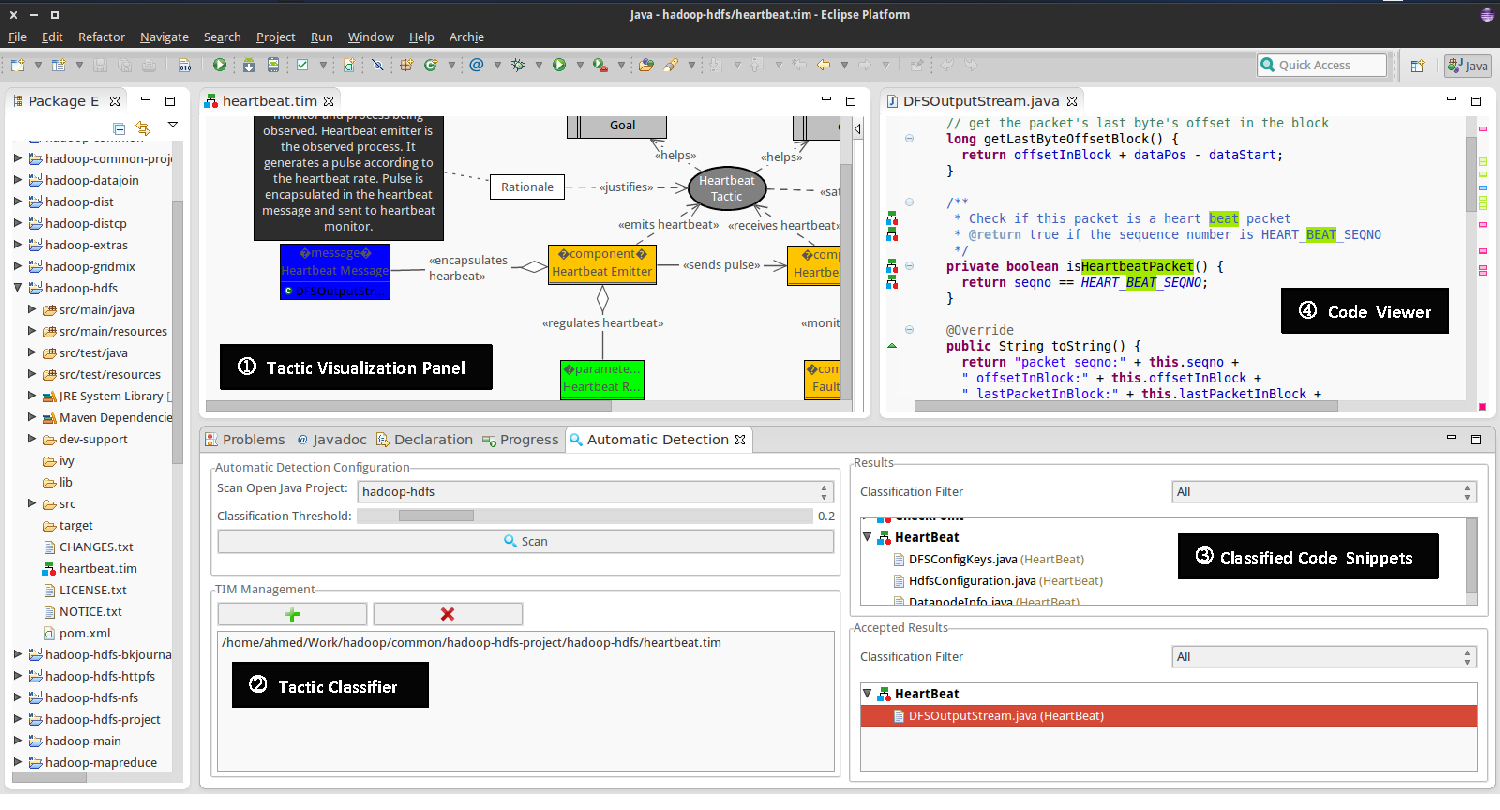
\includegraphics[width=0.9\linewidth]{./EclipseView}
\caption{A screen-shot of Archie, depicting different features and dashboards}
\label{fig:EclipseView}
\end{figure}


